\chapter{Granularity}
\label{chap:granularity}
As anyone in requirements engineering would state, the way requirements are stated matters. In the AADL/AGREE/Safety Annex approach of system development and safety assessment of models, we capture these requirements in \emph{guarantees} and \emph{assumptions} for the system components and the safety property is written as a top level guarantee or lemma. The process of verification proceeds by attempting to prove the safety property by use of the guarantees and assumptions at the lower system levels. A question that has come up in previous research work is how the formulation of the guarantees can affect the IVC analysis results~\cite{ghassabani_2018}. 

As described in Chapter~\ref{chap:prelim}, a transition relation is considered to be a conjunction of Boolean formulas. The granularity of these formulas will substantially affect the analysis results. Depending on how contracts are specified in the model, it is possible to have a ``complete" specification, i.e., all of the equations in the model are required to determine the validity of the property. However, in certain cases, subexpressions of equations may be irrelevant. If the equation is decomposed into smaller pieces, this incompleteness becomes visible and the model is no longer completely covered.\footnote{Simply put, coverage is a metric that determines how well properties cover the design of a model.} It is often the case that splitting an equation of the model into more conjuncts, or equivalently, making the model more \textit{granular}, leads to lower coverage of the model. This would be reflected in the IVCs generated for a given safety property; the IVCs in a more granular model would theoretically reflect only the necessary equations required for property verification, and thus would provide more specific analysis results.

Interestingly, similar work  from a varied perspective has been done in test case generation, specifically \emph{Modified Condition and Decision Coverage} (MC/DC). It was found that MC/DC over implementations with structurally complex Boolean expressions are generally larger and more effective than MC/DC over functionally equivalent but structurally simpler implementations~\cite{gay2016effect}. An automated technique called \emph{inlining} provides a restructuring of the model by inlining simpler Boolean expressions into a single, now more complex, expression. An example of an unlined implementation is: 

\begin{figure}[h]
	\begin{center}
		\includegraphics[scale=1.0]{images/uninlinedEx.PNG}
	\end{center}
	\vspace{-1.5em}
	%\caption{Uninlined implementation example}
	%\label{fig:uninlined}
\end{figure}

And the associated inlined implementation is: 

\begin{figure}[h]
	\begin{center}
		\includegraphics[scale=1.0]{images/inlined.PNG}
	\end{center}
	\vspace{-1.5em}
	%%\caption{Inlined implementation example}
%	\label{fig:inlined}
\end{figure}

Inlining results in a behaviorally equivalent implementation with different structure (syntax). The reason MC/DC provides much greater coverage in terms of test case generation is because MC/DC on an inlined system will require specific combinations of input that will not be required to achieve coverage of the noninlined system~\cite{gay2016effect}. 

Inductive validity cores, on the other hand, attempt to answer a different kind of question about the model than test coverage. In the IVC case, the goal is to find the minimal sets of model elements that contribute to a proof of a safety property. When these model elements are pulled from the model in terms of guarantees and assumptions, the \emph{granularity} of these logical statements matters in the opposite way. The IVC algorithm performs no deeper traces than those defined in those model elements (guarantees/assumptions). For our purposes, it is beneficial at times to see which \emph{parts} of the contract are necessary for the proof. In this case, instead of making the contracts more complex (inlining), we wish to simplify the contracts (un-inlining). In this way, the IVCs are more specific with regard to which parts of the contract are vital to the proof.

Granularity of contracts for IVCs has been previously discussed by Ghassabani~\cite{ghassabani_2018}, but to our knowledge has not been discussed in any other previous work -- in particular related to minimal cut set generation. Since IVC generation is a required first step of our minimal cut set algorithms, it is important to discuss how the granularity of the model will affect the cut sets generated through this approach. 

As described in Chapter~\ref{chap:mcsGen}, the backend model checker used in this transformation is \jkind which performs $k$-induction over a transition system defined with a Lustre program. Ghassabani did a preliminary investigation of granularity within the context of the Lustre language which provides a nice formalism for this discussion because it is top-level conjunctive, equational, and \textit{referentially transparent}~\cite{Halbwachs91:IEEE}. This means that the behavior of a Lustre program is defined by a system of equations and any subexpression on the right side of an equation can be extracted and assigned a fresh variable\footnote{A fresh variable is a variable with an identifier that has not been used within the program.} which is substituted into the original equation without changing the meaning of the program. In this context, \textit{granular refinement} is defined as an extraction of a subexpression into a new equation assigning a fresh variable. 


\section{Illustrative Example}
\label{sec:granularityEx}
To see how different representations of the system requirements will alter the MIVC and minimal cut set computations, let us examine once again the simple sensor example system that was described in Chapter~\ref{chap:compFF}. In this simple AADL architecture, the environmental temperature and pressure is sent to a subsystem of sensors which contains a temp sensor and a pressure sensor, both of which receive the respective environmental inputs. If the temperature (or pressure) surpasses a given threshold, then the temp (pressure) sensor outputs a high indication. It also gives the temperature (pressure) reading seen at the sensor. A diagram showing the two levels of the AADL implementation is shown in Figure~\ref{fig:sensorGran1}.  

\begin{figure}[h]
\begin{center}
\includegraphics[width=14cm]{images/sensorGran.png}
\caption{Tempurature Sensor System} 
\label{fig:sensorGran1}
\end{center}
\end{figure}

Now that the basic architecture is in place, we focus our attention on the requirements of each component. The behavior we wish to enforce at the temperature sensor level corresponds to the following two guarantees, $G_1$ and $G_2$. (Note: pressure sensor behavior is quite similar and for this reason, we will stick to the temperature for this example.) 

$G_1$: If environmental temperature surpasses threshold, then output high temperature indication: \textit{(temp $>$ THRESHOLD) $\implies$ (high\_temp\_indicator)}

$G_2$: Temperature read is equivalent to temperature in\footnote{We ignore noise in the temperature reading for simplicity's sake.}: \textit{temp = temp\_reading} 


These can be seen in the model as two distinct guarantees over the output of the sensor component. Now, as the contracts work their way up the system, there are distinct ways of writing them. For this, we will look to two metaphorical engineers who will provide the higher layer contracts to us. Let us assume that system A is built by engineer A. The top level safety property states: 
\begin{center}
    \textit{If environmental temperature reaches 90 degrees, then system reports high temperature.}
\end{center}

The direct subcomponent is the sensor system which contains the outputs: (1) a high temp indicator, and (2) the actual temperature. Engineer A chose to write the supporting contract in the subsystem as follows: 
\begin{center}
    $(T \geq 90 \implies temp\_high) \land (temp\_indicator = T)$ 
\end{center}
  
The example temp sensor system contract hierarchy is shown in Figure~\ref{fig:granularityEx1}.  

\begin{figure}[h!]
\begin{center}
\includegraphics[width=10cm]{images/granularityEx.PNG}
\caption{Temp Sensor System Contract Part I} \label{fig:granularityEx1}
\end{center}
\end{figure}

The safety property at the top level requires the contract $g_A$ for proof of validity. Thus, the \aivcalg should contain the contract $g_A$ as an MIVC. 

There are two faults defined for the temperature subsystem; one for each of the outputs. Fault $f_1$ affects the $temp\_high$ output and fault $f_2$ affects the $temp\_out$ output. Since each of these faults will violate the contract $g_A$, each of them will be found in the minimal cut set for $G_A$.

Now assume that Figure~\ref{fig:granularityEx2} was the system contract representation built by engineer B. 

\begin{figure}[h!]
\begin{center}
\includegraphics[width=10cm]{images/granularityEx2.PNG}
\caption{Temp Sensor System Contract Part II} \label{fig:granularityEx2}
\end{center}
\end{figure} 

The behavior and architecture of the system is the same, but the contract for the subsystem is more \textit{granular}; it is stated as two separate contracts:
\begin{center}
    $ g_A = (T \geq 90 \implies temp\_high)$ \\ 
    $ g_B = (temp\_indicator = T)$ 
\end{center}

Since $g_B$ is not required for the proof of either the system safety property nor the subsystem level property, only $g_A$ is found in the \textit{MIVC}s and thus only $f_1$ will be seen in the minimal cut set for this particular contract. 
 
In this simple example, it is easy to see how the granularity of the contracts may greatly affect the results of analysis. Structurally (syntactically), the contracts written by engineer A and engineer B vary; yet logically they are equivalent. The proof of the nominal system holds in both cases. Yet based on the architecture of the model and the formalization of the contracts, analysis results may be different. 

In the remainder of this chapter, we attempt to explore this problem through automation of contractual refinement and comparison of analysis results for both inductive validity cores and minimal cut sets. 
\section{Algorithms and Results}
The exploration of contractual granularity and its effect on analysis results was performed through the automation of contractual refinement. The algorithms and descriptions of results can be found in the following two subsections.. %All experimental results were run on a group of \danielle{describe benchmarks}.

\subsection{Initial Contractual Refinement}
\label{sec:granularityANDAlg}
The simplest restructuring that could be done on the model was to split any guarantees containing an $\land$ at the highest level of the Boolean formula and create additional guarantees from this refinement. The analysis performed on the model treats all guarantees as a large conjunction. This enables one to automatically split guarantees with expressions containing at the top level a conjunctive operator into two separate expressions. For instance, if $g_0 = A \land B$, then split this into $g_1 = A$, and $g_2 = B$ and insert $g_1$ and $g_2$ into the model and remove $g_0$. This was an initial probing of a deeper issue and gave a preliminary look into our assumption regarding minimal cut set generation in a model similar to that described in Section~\ref{sec:granularityEx}. Algorithm~\ref{alg:splitAnd} shows this algorithm used in this investigation. 

\begin{algorithm}[h]
\SetKwFunction{FMain}{$splitOnAnd$}
 \SetKwProg{Fn}{Function}{:}{}

	\Fn{\FMain{expression}}{
		Program $P$ \;
		Guarantees $list_G$ \;
		\For{all $g \in list_G$}{
			\If{binary statement with operator $\land$}{
			    insert into $P$ $\rightarrow$ new guarantee (left) \;
			    insert into $P$ $\rightarrow$ new guarantee (right) \;
				\FMain(left) \;
				\FMain(right) \;
			} %end if there exists AND in G
		}%end for all g in P
	}
	\caption{Split guarantees on logical $\land$ operator}
	\label{alg:splitAnd}
\end{algorithm}

The sensor described in Section~\ref{sec:granularityEx} is encoded into Lustre originally had a single guarantee as shown in Figure~\ref{fig:lustreOneGuar} that contained two subexpressions -- one of which was unrelated to the proof of the safety property.

\begin{figure}[h!]
\begin{center}
\includegraphics[width=1.0\textwidth]{images/lustreTwoGuar.PNG}
\caption{Temp Sensor With Original Guarantee} \label{fig:lustreOneGuar}
\end{center}
\end{figure}
 
Given the property \texttt{((env\_temp $>$ 8) $=$ high\_temp\_indicator)}, in the first case, \texttt{GUARANTEE0} is an MIVC for the safety property. Since both the fault defined on the temperature indicator and the fault defined on the temperature reading output affect \texttt{GUARANTEE0}, the minimal cut sets contain both faults. 

We then ran JKind on the model using Algorithm~\ref{alg:splitAnd}. The results of the algorithm on the Lustre encoding of the temperature sensor can be seen in Figure~\ref{fig:lustreTwoGuar}. 

\begin{figure}[h!]
\begin{center}
\includegraphics[width=.8\textwidth]{images/lustreOneGuar.PNG}
\caption{Temp Sensor With Modified Guarantees} \label{fig:lustreTwoGuar}
\end{center}
\end{figure} 

 In the second case, only \texttt{GUARANTEE2} is the IVC for the property. The minimal cut sets produced reflected what we expected and show only the high temperature indicator fault for the analysis in Figure~\ref{fig:lustreTwoGuar}. 

While this algorithm is efficient and quite simple, iit only addresses the case of a conjunction as the top level operator of the guarantee. Due to the logical nature of how the Lustre model is analyzed, all guarantees are viewed as a conjunction; therefore, splitting guarantees into new statements only works on the $\land$ operator. This is sufficient for illustration and an initial test into the problem, but cannot provide much decomposition in a general model. 

\subsection{Results of Initial Contractual Refinement}
\label{sec:resultsAND}
The initial contractual refinement was implemented in the safety annex and performed over the AGREE nominal guarantees. We tested the 18 AADL models used in Section~\ref{sec:timing} and compared the timing results of compositional verification without granular refinement and with this algorithm. The results can be seen in Figure~\ref{fig:graphGranularityAND}\footnote{All following analyses were run on an Intel Core i7 with a 2.80GHz CPU and 16 GB RAM. }. 

\begin{figure}[h!]
\begin{center}
\includegraphics[width=.8\textwidth]{images/graphGranularityAND15Models.PNG}
\caption{Nominal Analysis and Initial Granularity Refinement} \label{fig:graphGranularityAND}
\end{center}
\end{figure}

In most cases, the time of analysis is not increased. This is partially due to the size of the model in terms of the number of contracts, but also due to the specifications themselves; if a model does not contain top level conjuncts in the guarantees, no refinement occurs and the number of contracts in the model remains constant between both forms of analysis. No additional fresh variables are added and the total number of guarantees are equivalent. From the set of AGREE and safety annex annotated models available, all but six had no changes to guarantees. The six models that were transformed by this algorithm are shown in Table~\ref{tab:guarNoANDRefinement}. This provides insight into the timing results of Figure~\ref{fig:graphGranularityAND}.

\begin{table}[htbp]
\begin{center}
    \begin{tabular}{ | l | l | l | l | l | l | l | }
    \hline
    \textbf{} & $m=7$ & $m=12$ & $m=15$ & $m=16$ & $m = 17$ 
		& $m=18$    \\ \hline \hline
    No. Guarantees in Original & 10 & 12 & 15 & 121 & 160 & 168   \\ \hline
    No. Guarantees in Refined & 12 & 16 & 19 & 135 & 188 & 196   \\ \hline
    \end{tabular}
    \caption{Number of Guarantees in Original and Refined Models}
    \label{tab:guarNoANDRefinement}
    \end{center}
\end{table}

Table~\ref{tab:guarNoANDRefinement} shows for each model number how many guarantees were in the original model compared to the number of guarantees after this initial refinement. When comparing analysis times shown in Figure~\ref{fig:graphGranularityAND}, the changes in analysis time are clear. For instance model number 18 had originally 168 total guarantees (all component instances and top level safety properties). Thirteen of these were further decomposed in this algorithm.  

Compositional fault analysis was run using the algorithms described in Chapter~\ref{chap:compFF}. There was only two models in which changes were reflected in the minimal cut sets. In both cases, the sizes of cut sets were decreased by running this analysis. In one case, it was the model described in Section~\ref{sec:granularityEx}. In the other case, it was the WBS model described in Section~\ref{sec:wbs}. Given these results, we chose to implement a deeper refinement in JKind and this way could view more closely the results of MIVC generation. 
\subsection{Deeper Granular Refinement}
\label{sec:granularityFRESHAlg}
The granularity of the minimal cut sets directly reflect that of the MIVCs. While we eventually may want this algorithm implemented in the safety annex, we chose to begin the refinement in JKind in order to explore granularity from the context of MIVC enumeration. Specific comparisons could be made in terms of the number of MIVCs enumerated, the size of the MIVCs, and the time of analysis. 

The Lustre programming language provides a good formalism for discussion because it is top-level conjunctive, equational, and \emph{referentially transparent}: the behavior or a Lustre program is defined by a system of equations, and any subexpression on the right side of an equation can be extracted and assigned to a fresh variable which is substituted into the original equation without changing the meaning of a program~\cite{Halbwachs91:IEEE,ghassabani_2018}. In this context, we can define a \emph{granular refinement} as an extraction of a subexpression into a new equation assigning a new variable. 

The maximal factorization of the model can be obtained by assigning each instance of a subexpression and each use of an input to its own variable. This results in a \emph{totally decomposed} Lustre model: (1) each computed (non-input) variable is used at most once in the right side of an equation, (2) each equation is either a single operator or a constant expression, and (3) each model input is directly assigned to one or more fresh variables and is not used elsewhere in the model~\cite{ghassabani_2018}.

Ghassabani performed a preliminary analysis on maximally factored models for IVC coverage and found that analysis performed significantly slower for proofs and the \ivcmust algorithm~\cite{ghassabani_2018}. For our purposes in safety analysis, our concern is the guarantees in the Lustre model; therefore, we are able to weaken the factorization performed. To this end, a \emph{partially decomposed} Lustre model has the properties that (1) each computed variable is used at most once in the right side of an equation, and (2) each equation has either a single operator or a literal as the right hand side. The reason we focus on these two properties is because the portions of the model that are of interest are the guarantees (Lustre equations) that constrain the output of a node and any equations these guarantees may reference. We were interested in two main research questions regarding the exploration of granularity refinement: 

\begin{description}
\item[RQ1:] Do the MIVCs generated reflect a more accurate view of which elements of the model support the proof of the safety property? We expect that the additional granularity would provide more exact information regarding which subformulae of a guarantee contribute to proof.

\item [RQ2:] What is the analysis time difference between the nominal model MIVC generation and the decomposed model MIVC generation? Given smaller models with fewer or less complex guarantees, the timing results should not differ greatly, but in a large model with potentially many complex guarantees, the computation time for MIVC generation could increase dramatically. 
 
\end{description}

To explore these questions, we developed an algorithm that performs a partial decomposition of the Lustre model. The logical structure of a formula can be viewed as a tree where nodes are arranged in terms of operator precedence. Clearly, semantic equivalence must be preserved during refactoring and we only want to change the structure (syntax) of the formula. To this end, we isolated branches and subtrees of the structure so that the \aivcalg algorithm can view each subtree of the formula separately. The algorithm recursively travels through a formula tree, assigning each subtree as a fresh variable. Figure~\ref{fig:formulaTree} shows the following formula in tree structure where \textit{lit} refers to a literal:
\begin{gather*}
((((\mathit{lit} \implies \mathit{lit}) \lor \mathit{lit}) \iff \mathit{lit} ) \land (\mathit{lit}  \lor \mathit{lit} )) 
\end{gather*} 

\begin{comment}
\begin{figure}
\begin{center}
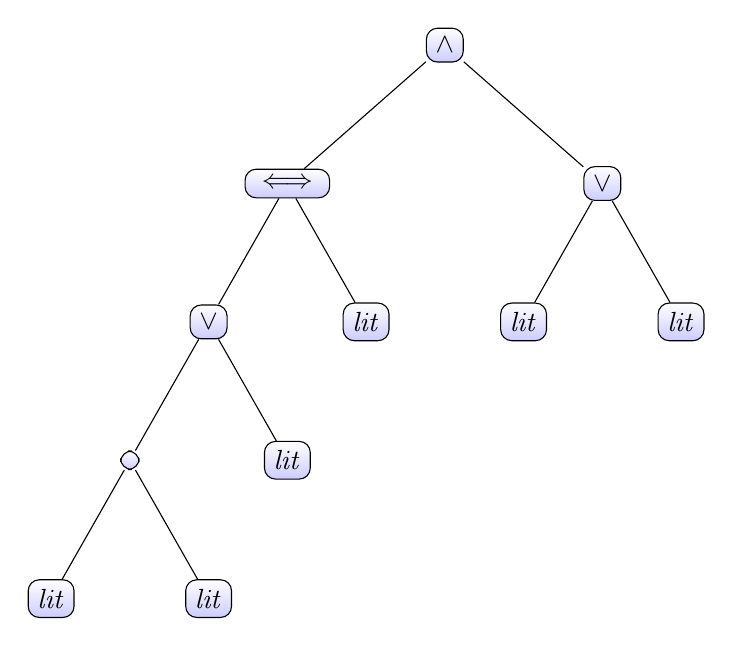
\begin{tikzpicture}[level distance = 5em, every node/.style = {shape=rectangle, rounded corners,
    draw, align=center,
    top color=white, bottom color=blue!20}]]
  \tikzstyle{level 1}=[sibling distance=40mm] 
  \tikzstyle{level 2}=[sibling distance=20mm] 
  \tikzstyle{level 3}=[sibling distance=20mm] 
\node {$\land$} 
    child { node {$\iff$} 
	  child{ node{$\lor$}  
 	    child{node{$\implies$} 
            	 child{ node{\textit{lit}}  } 
	          child{ node{\textit{lit}}  }   
 	    }
 	    child{node{\textit{lit}}}	  
	  }
	  child{ node{\textit{lit}}  }    
    }
    child { node {$\lor$}
      child { node {\textit{lit}} }
      child { node {\textit{lit}} } } ;
\end{tikzpicture}
\end{center}
\caption{Graphical Representation of a Boolean Formula}
\label{fig:formulaTree}
\end{figure}
\end{comment}

\begin{figure}[h!]
\begin{center}
\includegraphics[width=.6\textwidth]{images/treeFormula.png}
\caption{Graphical representation of a Boolean formula} 
\label{fig:formulaTree}
\end{center}
\end{figure} 

As seen in Figure~\ref{fig:formulaTree}, the leaf nodes of the tree are literals; these are the base cases in the recursion. The formula provided as an example has only binary operators; in the algorithm used for refactoring the Lustre equations, unary, binary, and tertiary (if-then-else) operators are handled in a similar fashion.

Each subformula is assigned a fresh variable and added to the equations for the Lustre node. The fresh variables are also assigned to be IVC elements and considered during the \aivcalg algorithm. This is the resulting equation (Figure~\ref{fig:formulaTree}) after refactorization:\\
\texttt{eqn\_name = (FreshVar0);}\\
\texttt{FreshVar0 = (FreshVar1 and FreshVar2);}\\
\texttt{FreshVar1 = (FreshVar3 = lit);}\\
\texttt{FreshVar2 = (lit or lit);}\\
\texttt{FreshVar3 = (FreshVar4 or lit);}\\
\texttt{FreshVar4 = (lit => lit);}

\subsubsection{RQ1}
We present a fictitious monitor component of a system as shown in Figure~\ref{fig:monitorLustre}. There are two components being monitored for validity (components A and B), each of which sends an error indication to the monitor, \texttt{errorCompA} and \texttt{errorCompB}. The monitor calculates  a \texttt{valid} indication if neither error indication is true and when \texttt{output} should be sent. There are two conditions in which the monitor is disabled: when a disable command is explicitly sent or when the system is not in auto mode. The property we wish to show is that the monitor does not calculate both a \texttt{valid} and \texttt{invalid} value simultaneously. 
\begin{figure}[h!]
\begin{center}
\includegraphics[width=.8\textwidth]{images/monitorLustre.PNG}
\caption{The Lustre Model of a Monitor} 
\label{fig:monitorLustre}
\end{center}
\end{figure} 

The MIVC generated for this property is: $\{$\texttt{valid}, \texttt{invalid}$\}$. Due to the simple nature of this model, it is clear to see that only the error indications from components A and B referenced in equation \texttt{valid} are directly used for the proof of the property, and the branch of \texttt{valid} that references \texttt{output} is not necessary. Since this equation is not sufficiently granular, the MIVC contains the entire \texttt{valid} equation. After performing the refactorization using fresh variables for the model equations, the Lustre code is transformed into what is shown in Figure~\ref{fig:monitorFreshLustre}. 
\begin{figure}[h!]
\begin{center}
\includegraphics[width=.8\textwidth]{images/monitorFreshLustre.PNG}
\caption{The Lustre Model of a Monitor After Refactorization} \label{fig:monitorFreshLustre}
\end{center}
\end{figure} 

The equations are broken down into their respective subformulae and refactored such that the equations are totally decomposed and semantically equivalent. While this adds a significant number of new variables and equations to the model, the MIVCs generated give more information on the subformulae of the equations necessary for proof. The MIVCs of the refactored model are shown in Figure~\ref{fig:monitorFreshIVCs}. 
\begin{figure}[h!]
\begin{center}
\includegraphics[width=.6\textwidth]{images/monitorFreshIVCs.PNG}
\caption{The MIVC of the Refactored Monitor Model} \label{fig:monitorFreshIVCs}
\end{center}
\end{figure} 

To preserve semantics of the equations during the decomposition, the original equation must be assigned a fresh variable. The MIVC algorithm captures the original equation in \texttt{FRESHVAR0}, but also provides a trace down the branch of the equation that is required for the proof. In this case, it traces down the left side of the original binary equation (\texttt{valid}) and chooses the fresh variable associated with: \texttt{not(errorCompA and errorCompB)}. This correlates to \texttt{FRESHVAR1}. Instead of only providing the equation \texttt{valid} as an MIVC, we see the necessary subformula required for the proof. The third MIVC in this case simply maps back to \texttt{invalid}. 

The MIVCs now provide information on the necessary subformulae of an equation and not only the equation itself. If all branches are required, then all associated fresh variables would be found in those MIVCs. To further explore this question, we also want to see how the sets themselves change after refactorization. To this end, we ran a set of Lustre benchmark models used in previous MIVC enumeration work~\cite{ghassabani_2018} and compared the original MIVC enumerations to the refactored model MIVC results in terms of both number of sets generated and the cardinalities of the sets. In some cases, more MIVCs were generated and in many cases, the MIVCs had greater cardinality. The reason is because every equation that is not assigned to only a literal is refactored and assigned fresh variables. 

\begin{figure}[h!]
\begin{center}
\includegraphics[width=1.0\textwidth]{images/xml_output.png}
\caption{XML MIVC analysis output comparison} 
\label{fig:xml_ivc}
\end{center}
\end{figure}

Figure~\ref{fig:xml_ivc} displays the output of a benchmark model. On the left is the MIVC analysis results for the orginal benchmark model and as a point of comparison, the results for the refactored model are shown on the right. For the original model\footnote{\texttt{\_6counters\_e3\_140\_e8\_149.lus}}, a single IVC of cardinality 5 is enumerated. After refactorization and analysis, the number of MIVCs increased. Depending on the equations necessary for proof of model safety properties, this varies considerably. In some cases, the resulting MIVCs only contain fresh variables corresponding to the original MIVC (cardinality is greater). In other cases, the MIVCs contain fresh variables that describe a subformula of the original results. 

\subsubsection{RQ2}
The refactorization described in the previous section introduces multiple new variables and equations into the Lustre model. While a more exact trace of each equation is possible using this method, the size of the model could grow substantially making the time of analysis unacceptable. We ran a subset of the Lustre benchmark models and compared the time difference between the MIVC enumeration of the refactored models and the MIVC enumeration of the original benchmark models without any refactorization. To use this approach for minimal cut set generation, both the refactorization and the MIVC enumeration must be performed. The total time of the algorithm provided in this chapter and the MIVC collection over the refactored models is used in the time comparison. We used Z3 as a solver and the only IVC elements flagged for consideration were the fresh variables. The timing comparison results are shown in Figure~\ref{fig:granIVC}. 

\begin{figure}[h!]
\begin{center}
\includegraphics[width=.8\textwidth]{images/granularityIVC2.png}
\caption{Timing comparison for generating MIVCs} 
\label{fig:granIVC}
\end{center}
\end{figure}

For many of the small benchmark models, the time difference between the original and refactored models is not significant. This is likely due to a relatively small number of additional equations inserted into Lustre. Although as can be seen in Figure~\ref{fig:granIVC}, the time of analysis seems to be entirely dependent on the model. All of the models used in this subset of Lustre benchmarks is analyzed using the \aivcalg algorithm in under 6 seconds. The time increase for refactorization varies between the original MIVC time and orders of magnitude higher. When analyzing some of these time intensive models, the reason was clear. The original models contained numerous equations and each equation introduced numerous additional fresh variables into the model.

To introduce a granularity option into the analysis for MIVC enumeration, minimal cut set generation, or other such analyses may provide valuable insight into the model, the specifications, and the faults that contribute to a top level hazard. 

\subsubsection{Future Work for Minimal Cut Sets}
Given the results in RQ2, could more exact minimal cut sets be produced from the MIVCs? If changes are reflected in the MIVC sets, then we will see corresponding changes in the minimal cut sets as shown in the preliminary investigation of Section~\ref{sec:granularityANDAlg}. This Would provide more exact safety analysis artifacts and additional insight into the specifications and how they impact the analysis results.

The method used in this algorithm provides all fresh variables to the MIVC algorithm. The results seen in the MIVCs reflect a branch of the Boolean equation. The transformation from MIVCs to minimal cut sets include a hitting set algorithm. Given the IVC results of this granularity algorithm, the hitting sets would split the branch shown in the MIVC such that the semantics of results would no longer be sound. In order to use these MIVCs for minimal cut set generation, he branch of a formula in an MIVC would need to be inlined before the hitting sets were computed. At that point, the single formula/branch could be used in the hitting set algorithm without loss of meaning. 

After this processing, the minimal cut sets could be found by mapping the subformula to a fault that violates the output referenced in that subformula. Further work is required to implement this approach, but given the preliminary findings of this exploration, this approach is promising to provide insight into model specifications, subformula necessary for proof, and more exact minimal cut sets. 







%\subsection{Mutations and Equation Removers}
For the development of model-based critical systems, it has been argued that formal proof should be applied to gain higher confidence in the model than with testing alone, e.g.~\cite{hardin2009development,miller2010software,rushby2009software,bozzano2003improving}. This has proven to be an active area of research, but has also shown some missing pieces -- one of which will be of benefit to us in this granularity exploration. When a property is proved valid, no further information is provided about the coverage of the model. One does not know whether the model contains features that are not covered by the properties~\cite{NFM2020Todorov}. Furthermore, we do not know if features \emph{within an IVC element in an MIVC set} are completely covered by the property. To this end, we began to look into mutation coverage to provide an answer. 

A mutation approach described by Todorov et al.~\cite{NFM2020Todorov} consists in mutating a model for which safety properties were proved valid, and trying to prove the same properties on the mutated models (\emph{mutants}). If the mutant is proved to be valid (i.e., it \emph{survived}), the mutant reveals part of the model that is not covered by the properties. We know that portion of the model is not necessary to find a proof. The approach described in this section attempts to use this type of mutant analysis on the contracts of a Lustre model, and thus compare to a granular refinement MIVC approach. 

A brief review of transition systems and some definitions are provided for convenience. 

Given a state space $U$, a transition system $(I,T)$ consists of an
initial state predicate $I : U \to \bool$ and a transition step
predicate $T : U \times U \to \bool$.
We define the notion of
reachability for $(I, T)$ as the smallest predicate $\reach : U \to
\bool$ which satisfies the following formulas:
\begin{gather*}
  \forall u.~ I(u) \Rightarrow \reach(u) \\
  \forall u, u'.~ \reach(u) \land T(u, u') \Rightarrow \reach(u')
\end{gather*}
A safety property $P : U \to \bool$ is a state predicate. A safety
property $P$ holds on a transition system $(I, T)$ if it holds on all
reachable states, i.e., $\forall u.~ \reach(u) \Rightarrow P(u)$,
written as $\reach \Rightarrow P$ for short. When this is the case, we
write $(I, T)\vdash P$.

The Lustre model is a set of equations$\{eq_1, \dots,eq_n\}$ and the transition relation $T$ has the structure of being a top level conjunction $T = t_1 \land \cdots \land t_n$ where each $t_i$ is an equality corresponding to $eq_i$. By further abuse of notation, $T$ is identified with the set of its top-level equalities. When an equation is removed from the Lustre model, an equality $t_i$ is removed from $T$ and the transition relation becomes $T\setminus \{t_i\}$. 

\begin{definition}
Minimal Inductive Validity Core (MIVC)~\cite{Ghassabani2017EfficientGO}: $S \subseteq T$ is a minimal Inductive Validity Core, denoted by $MIVC(P,S)$, iff $IVC(P,S) \land \forall T_i \in S$. $(I, S \setminus \{T_i\}) \not \vdash P$.
\end{definition}

In this research, we are only interested in minimal sets that satisfy a property $P$; if $(I, T) \vdash P$, then we know $P$ always has at least one MIVC which is not necessarily unique. By computing all MIVCs, we have a complete mapping from the requirements to the design elements; this is called \emph{complete traceability}~\cite{murugesan2016complete}. 

Ghassabani defines two metrics of coverage~\cite{ghassabani2017proof}. 

\begin{definition} \maycov\ : $t \in T$ is covered by $P$ iff $t_i \in $\maycov$(P)$, where \maycov$(P) = \{t_i | \exists S \in AIVC(P) \cdot t_i \in S\}$.
\end{definition}

\begin{definition} \mustcov\ : $t \in T$ is covered by $P$ iff $t_i \in $\maycov$(P)$, where \maycov$(P) = \{t_i | \forall S \in AIVC(P) \cdot t_i \in S\}$.
\end{definition}

The \maycov\ elements are relevant to the proof, but may be modified without affecting the satisfaction of $P$, whereas the \mustcov\ elements are absolutely necessary for the proof of $P$. One can view the \mustcov\ set of elements as the intersection of all MIVCs; if a single \mustcov\ element is removed, it ``breaks" all proofs of $P$. 

A mutator is formally a function that mutates any transition predicate $T$ to a set of mutants $\{T^1_{mut}, \dots, T^m_{mut}\}$, where each mutant $T^i_{mut}$ is obtained by applying a change to $T$. A very simple mutator is one that simply removes an equality $t_i$ from $T$, which amounts to removing the corresponding line of code from the Lustre model~\cite{NFM2020Todorov}. Todorov et al.~\cite{NFM2020Todorov} implemented an \emph{equation remover} in JKind which removes equations one by one and replays the proof process in an incremental way. If after removing an equation, the properties are still proved (the mutant survives), it means that the removed equation has no impact on the proof. If the properties do not hold any longer (the mutant is killed), then we know the removed equation is essential for the proof. This mutator computes the minimum \mustcov\ core. 


%\subsection{Mutations and Guarantees}
\label{sec:granularityMutationInputs}
In the early stages of safety analysis on a complex critical system, it is beneficial to see what model elements may contribute to a property violation. While it is true that analysts will define faults based on their knowledge of the domain, at times in complex systems not all of these faults and their consequences are clear. Using the idea of mutations, we wish to see what the critical inputs to a system may be. 

As an example, we look once again at the sensor subsystem of a PWR as outlined in Chapter~\ref{chap:mcsGen}. Given a nominal system model containing the sensor subsystem and a single temperature sensor, we wish to see what model elements -- specifically guarantees -- are the \mustcov\  elements for the program. This tells the analyst that if these guarantees are violated, there are no paths to a proof of the property. 

To this end, we modified the equation remover implemented by Todorov, et al.~\cite{NFM2020Todorov} in JKind in order to collect killed guarantees from the program in Lustre. The results from the modified equation remover shows the following guarantees that are critical to any proof (Figure~\ref{}). 

After finding these results, we then defined a fault on the output governed by this guarantee and ran the minimal cut set generation on the fault model. As expected, this fault was in the minimal cut sets. While this example is sufficiently simple to illustrate the point, in complex models there can be multiple guarantees for a single component, many different components in a subsystem all of which are connected in various ways. It is obvious to anyone looking at the sensor subsystem model that this particular fault will violate the property. To this end, we turned our attention to a larger model: the Wheel Brake System as described in Section~\ref{chap:wbs}. At the time of this analysis, there were XX faults defined for XX components throughout the extended system model. The total number of contracts of the nominal model exceeded XXX. We ran this analysis to see if there were other faults that may have been overlooked during the development of the WBS model. 

A guarantee on the XX component was presented in the mutation analysis: \danielle{FIGURE OF GUARANTEE AND DESCRIPTION}. 

We defined a fault for the XX component as shown in Figure\danielle{make me}. Running minimal cut set generation with the additional constraint of one active fault, this fault is seen in the minimal cut sets; the violation of the property occurs when this fault is present. 

Performing a kind of mutation analysis could be beneficial during the fault modeling process to catch things that may be missed during the fault definition process. The initial foray into mutation testing results show that this has potential for integration into the safety annex. It was also clear that a better representation was needed for large models. In the case of the WBS mutation analysis, over XX guarantees were given as candidates for faults -- many of which already had faults associated with them. By integrating this feature into the fault analysis, these guarantees could be pruned from the output and save the user from pouring through potentially hundreds of guarantees. 

\subsection{Node Inputs and Mutation Testing}
The equation remover mutation also iterates through Lustre node inputs and performs the mutation one input at a time. The node inputs in the Lustre model correspond to the inputs and outputs of an AADL component as shown in Figure~\ref{fig:nodeInputsLustre}. 

\begin{figure}[h]
	\begin{center}
		\includegraphics[scale=0.8]{images/nodeInputsLustre.PNG}
	\end{center}
	%\vspace{-1.5em}
	\caption{An AADL Component and Lustre Node Inputs}
	\label{fig:nodeInputsLustre}
\end{figure}

Given that the equation remover algorithm can perform this operation over node inputs, we can also gather information about critical outputs of components. Performing a similar extention to the equation remover algorithm, we collected all node input mutations that are killed and present them to the user. As an example, we show in Figure~\ref{fig:nodeInputsKilled} the analysis results on the nominal temperature subsystem example. 

\begin{figure}[h]
	\begin{center}
		\includegraphics[scale=0.6]{images/nodeInputsKilled.PNG}
	\end{center}
	%\vspace{-1.5em}
	\caption{Temperature Node Inputs Killed by Equation Remover}
	\label{fig:nodeInputsKilled}
\end{figure}

Given that there exists an assumption on the temperature sensor input, we focus on the output. The only killed output was that of the high temperature indication, which tells us to prove the guarantee $\mathit{env\_temp} > 8 \iff \mathit{temp\_high}$, the output of this node is of utmost importance. Not surprisingly, when attaching a fault to this output, we get this fault in the minimal cut set for the top level property. 

As in the case with application of mutation testing on guarantees, node inputs also will require integration into the safety annex in order to filter out node inputs that have already been accounted for with faults in the extended system model. In large systems, this analysis is scalable and shows itself to be informative, but the outputs are unwieldy and large. Further work to rectify this would be required before use in large systems. 

The investigations into mutation testing applied to fault analysis were implemented in JKind and can be found at \url{https://github.com/dkstewart/jkind} on the {\em fault\_analysis\_mutations} branch.


